\subsection{Design}


\subsubsection{Scenarios}

Since milestone 3 VFS Browser can run in two different modes. Classic
mode\ref{fig:scenario_classic_mode} basically is the usage of virtual disks without any
server involved. Sync mode\ref{fig:22scenario_sync_mode} allows propagating
changes on a local disk (step 1) to a server (step 2). In
this mode changes are recorded in a journal, that gets sent over the wire when
the ``sync'' button is hit. To use a disk in sync mode one has to link a disk to
a server so that synchronization takes place between the local disk and the disk
on the server. The mechanism of journaling allows offline usage of a linked
disk, so that later on, when reconnecting to a server, local changes get
propagated to the disk on server side. Such changes on the
server side are sent to freshly attached clients that are working on the same
linked disk.

\begin{figure}[h!]
\centering
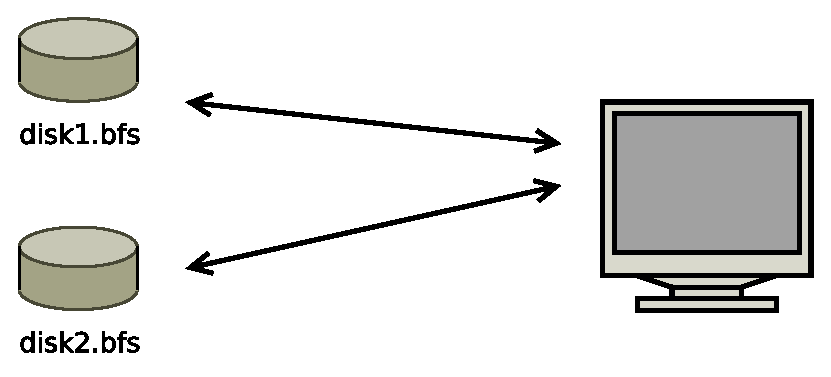
\includegraphics[width=1\textwidth]{figures/22scenario_classic_mode.eps}
\caption{scenario classic mode}
\label{fig:scenario_classic_mode}
\end{figure}

\begin{figure}[h!]
\centering
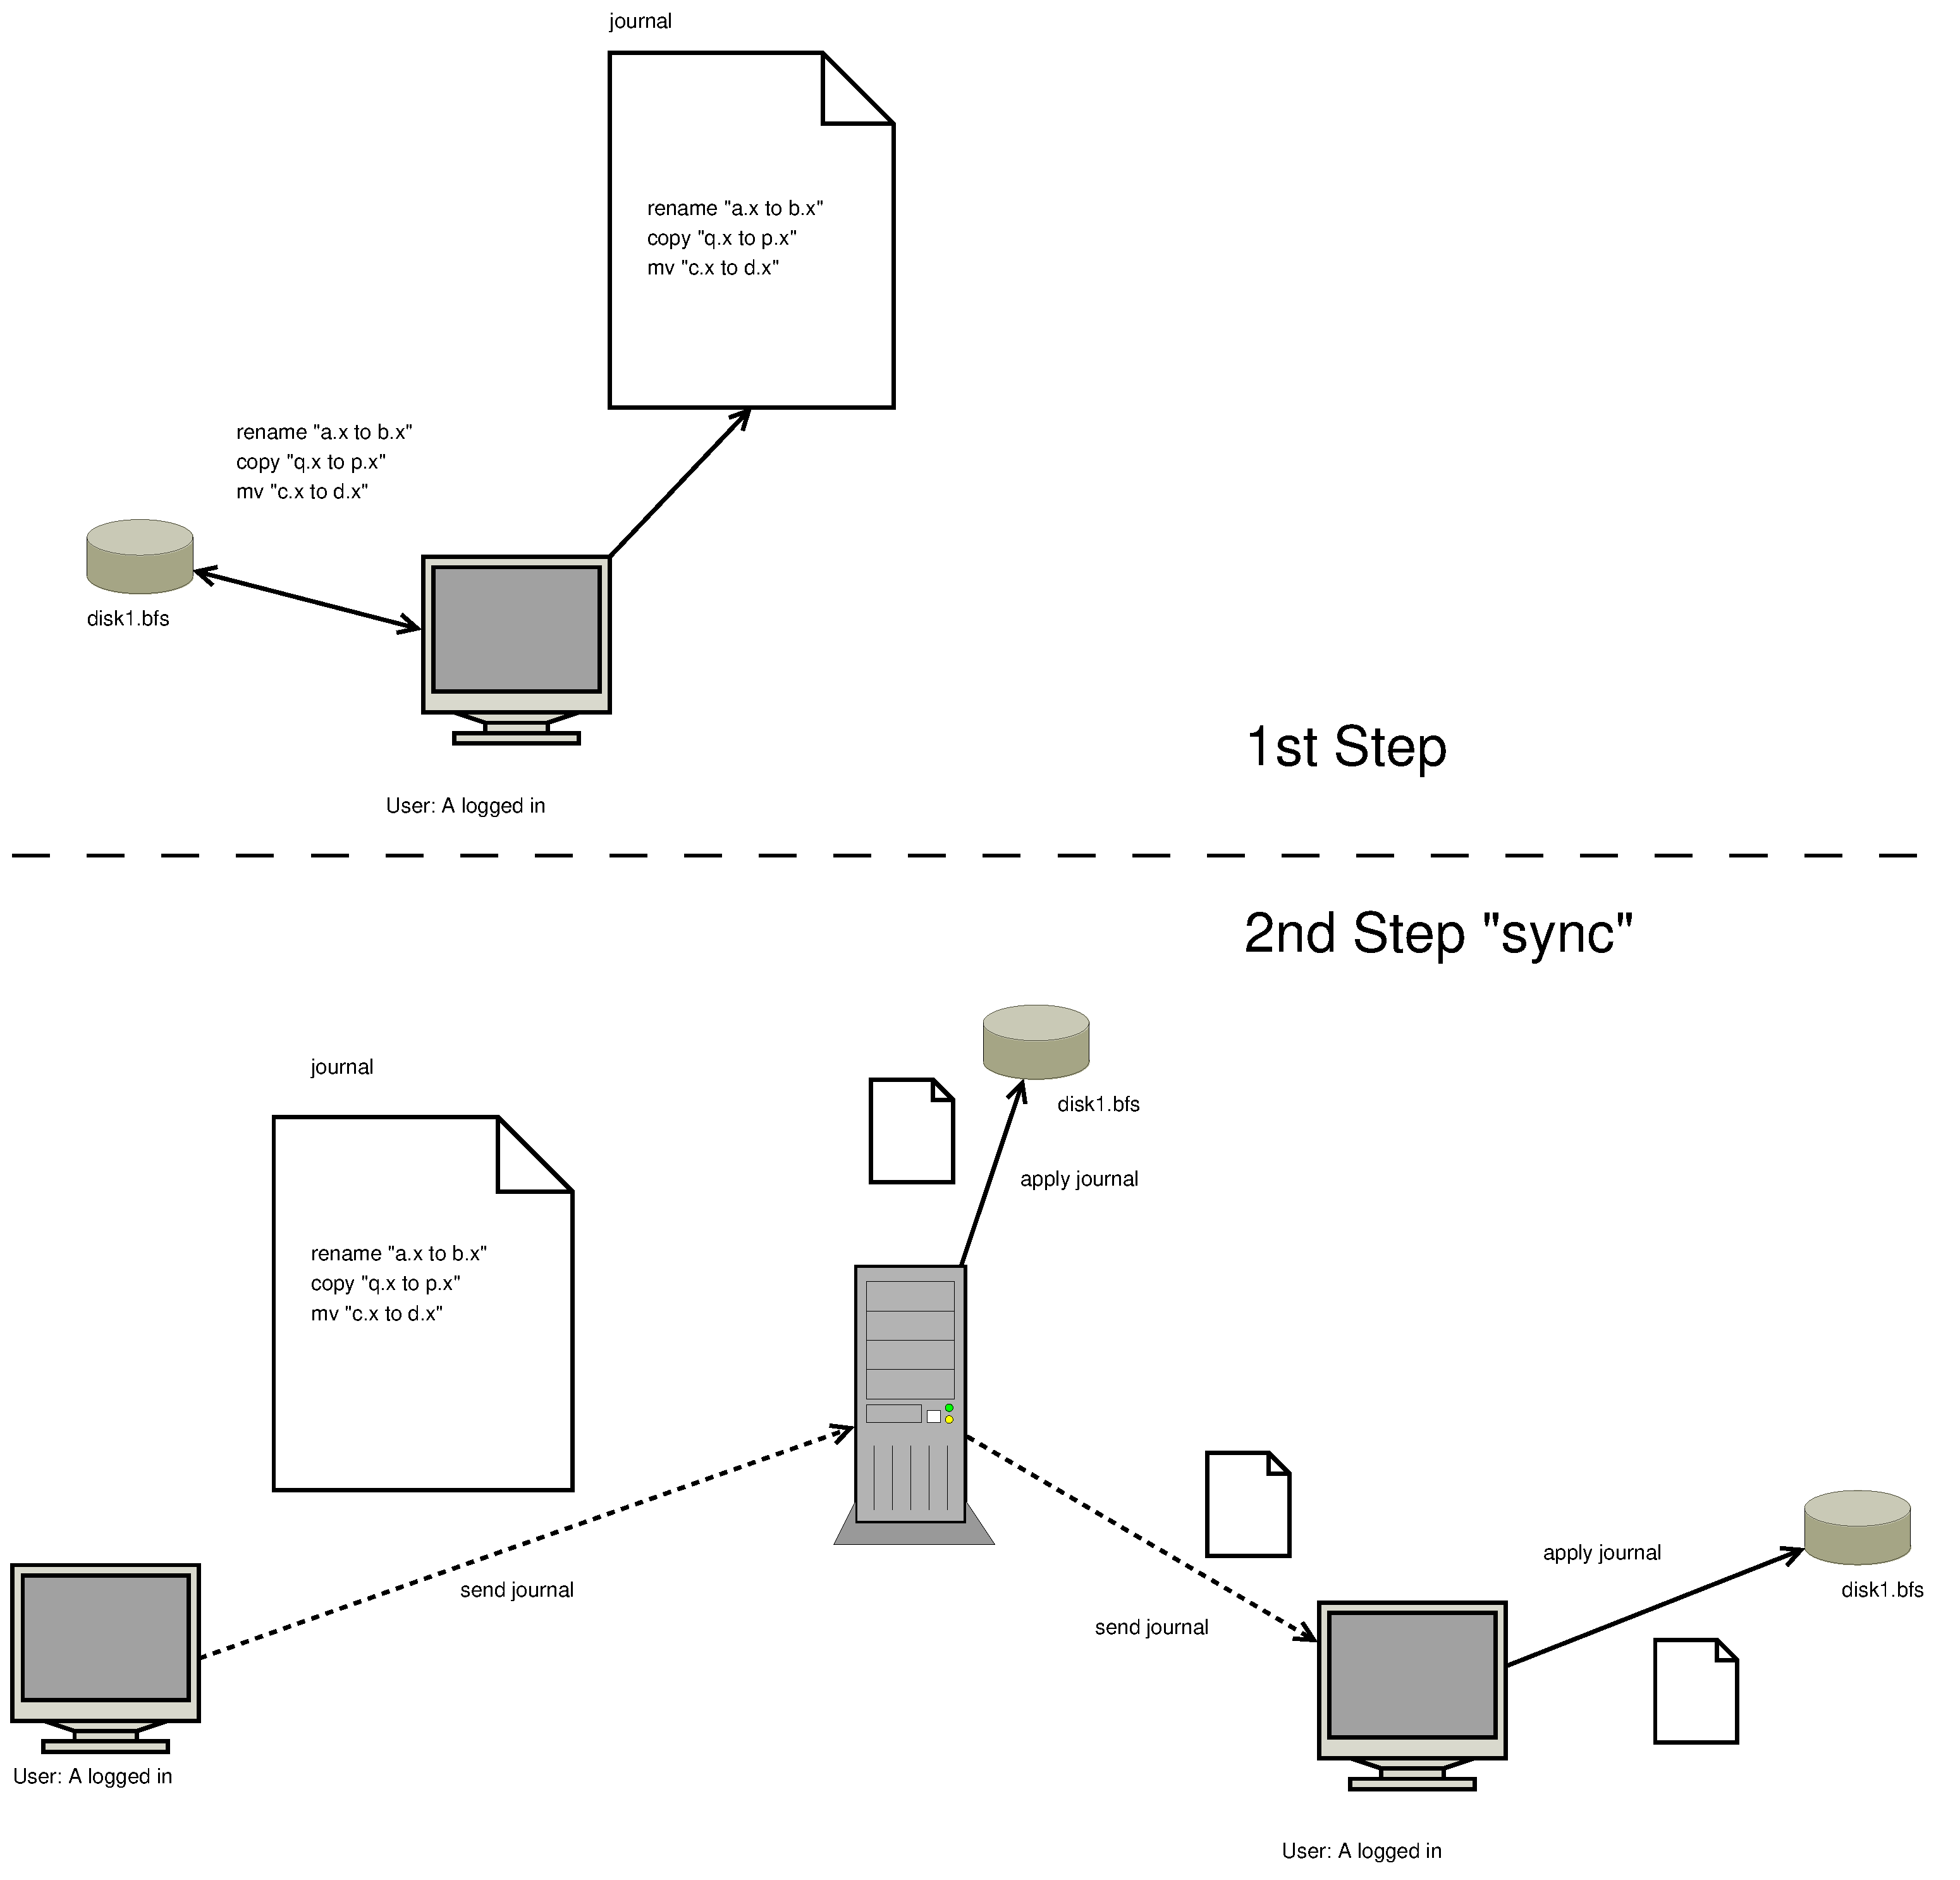
\includegraphics[width=1\textwidth]{figures/22scenario_sync_mode.eps}
\caption{scenario sync mode}
\label{fig:22scenario_sync_mode}
\end{figure}

\subsubsection{Technology}

\begin{figure}[h!]
\centering
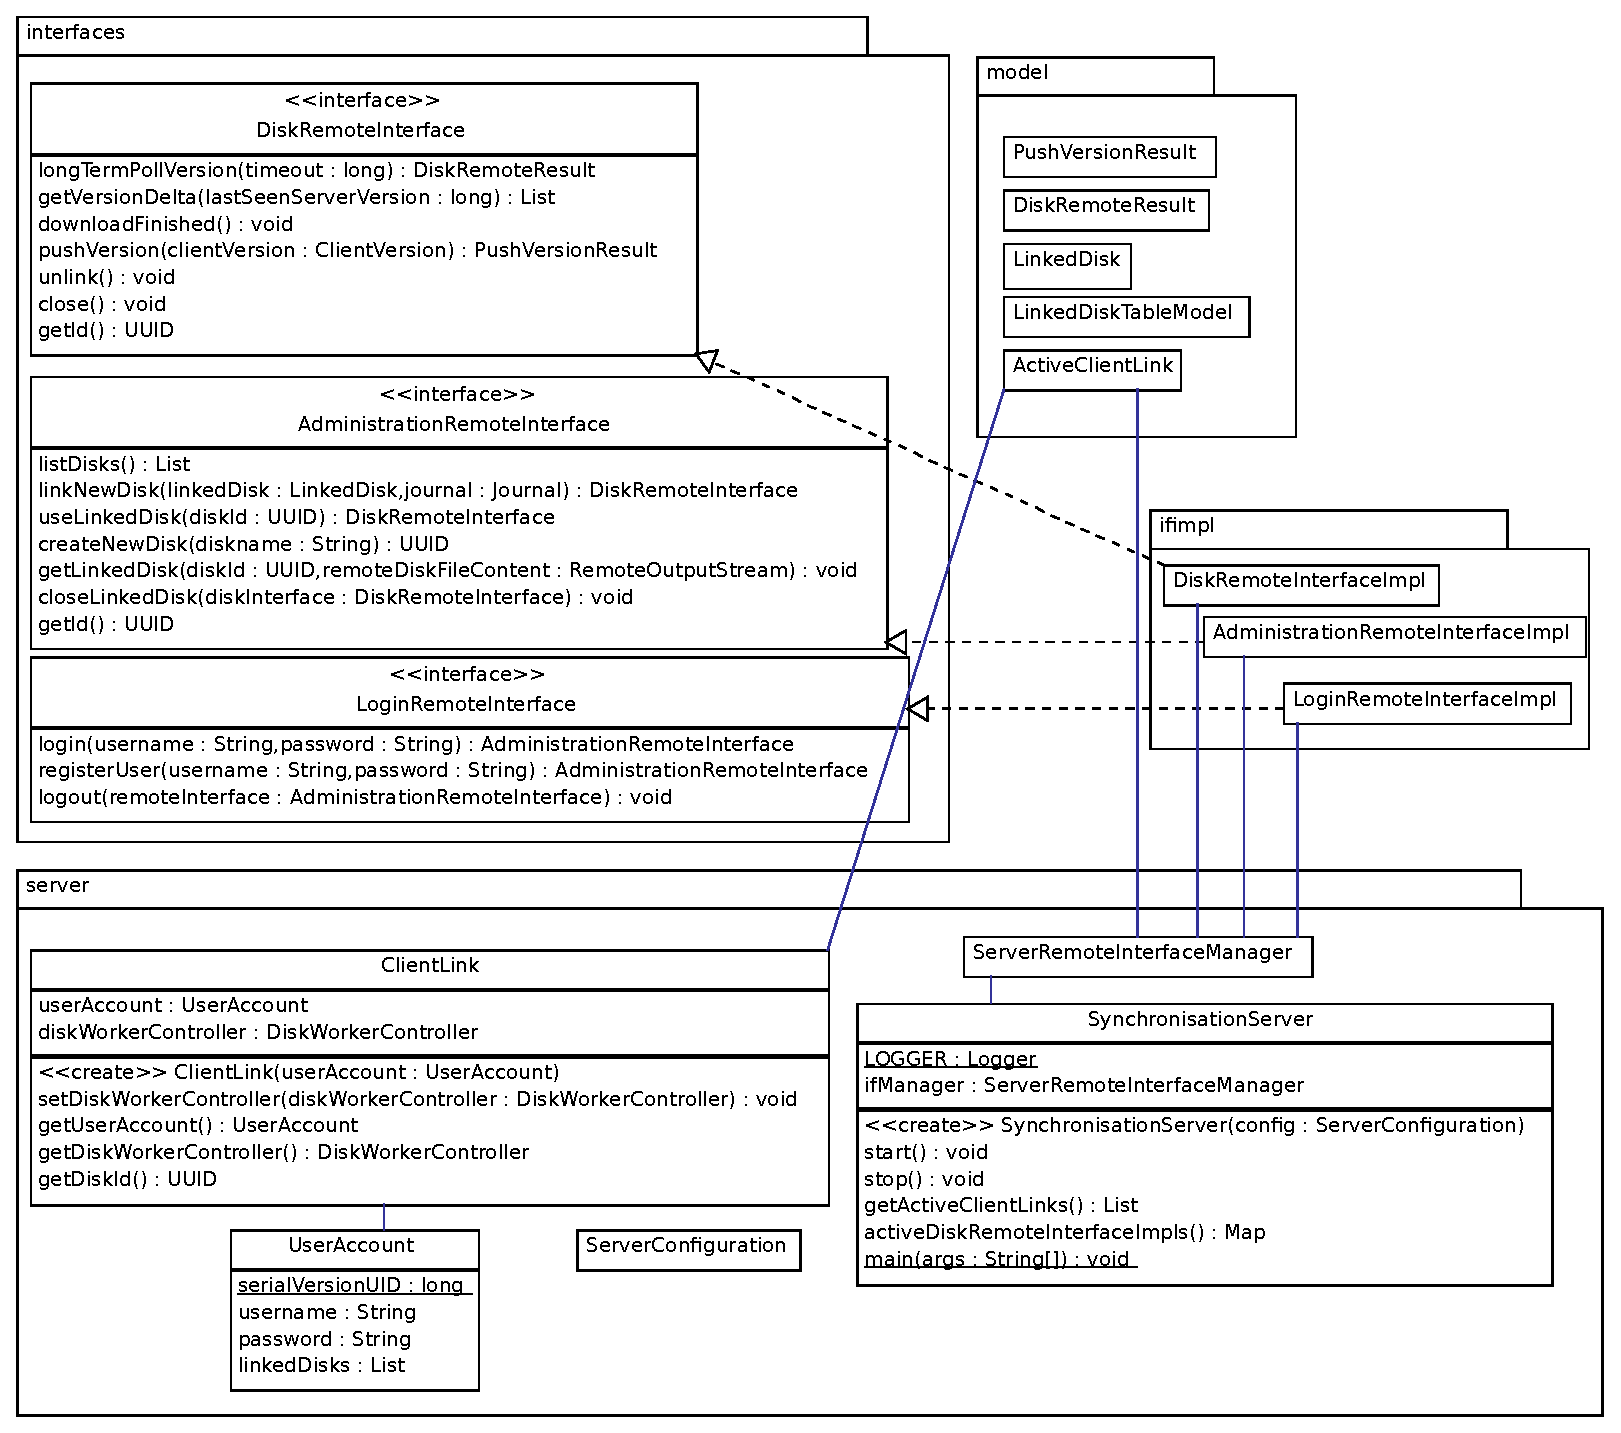
\includegraphics[width=1\textwidth]{figures/22Server.eps}
\caption{Server classes}
\label{fig:22server_classes}
\end{figure}

It was chosen to use JAVA RMI to establish client server
communication. Figure \ref{fig:22server_classes} shows the interfaces and
classes, that werde implemented to achieve communication. The three interfaces
\textit{LoginRemoteInterface, AdministrationRemoteInterface,
DiskRemoteInterface} hide the functionality to login/logout, create/link disks,
and push/pull journal updates for a disk. When a server startes up the
\textit{LoginRemoteInterfaceImpl} gets registered into the RMI registry and from
now on clients are allowed to connect through its interface. Every time a
client successfully logs in to the server a new
\textit{AdministrationRemoteInterfaceImpl} gets instantiated so that the client can link or open disks. Every time a disks
gets opened a new instance of \textit{DiskRemoteInterfaceImpl} gets
instantiated through which the client can synchronize local changes to the
corresponding server disk.


\subsubsection{User Management}
User management is kept very simple. Upon connecting to a server one can
create a new username/password or use a already existing one. Credentials are
being saved on server side together with its linked disks (see
\textit{UserAccount}).

\subsubsection{Synchronization}
Synchronization of disks is achieved by a simple journaling mechanism. Journals
get recorded when changes on a linked disk are made. These recorded journals get
sent to the server when ``sync'' button is hit. Changes that were done on a
remote client get synchronized to the local client uplon login or periodically
with a long term polling mechanism. Figures \ref{fig:22uploadChanges} and
\ref{fig:22downloadChanges} show roughly, what happens when the ``sync'' button
is pressed: Through some indirection (\textit{DiskWorkerController and
RemoteWorkerController} that allow loose coupling of GUI, local disk and remote
communication threads) the client uploads/downloads \textit{Journal}s containing
\textit{JournalItem}s to/from the server which then get replayed on the other
side. Notice in particular the \textit{ModifyFileItem} that carries a special
veriant of \textit{InputStream} to copy the binary data from a file to the other
side. A small drawback of this design is that while client is doing
synchronization no other actions can take place on its local disk. This includes
changing folder or simply all reading actions. Due to the lack of time it was
decided not to investigate further on that topic.

\begin{figure}[h!]
\centering
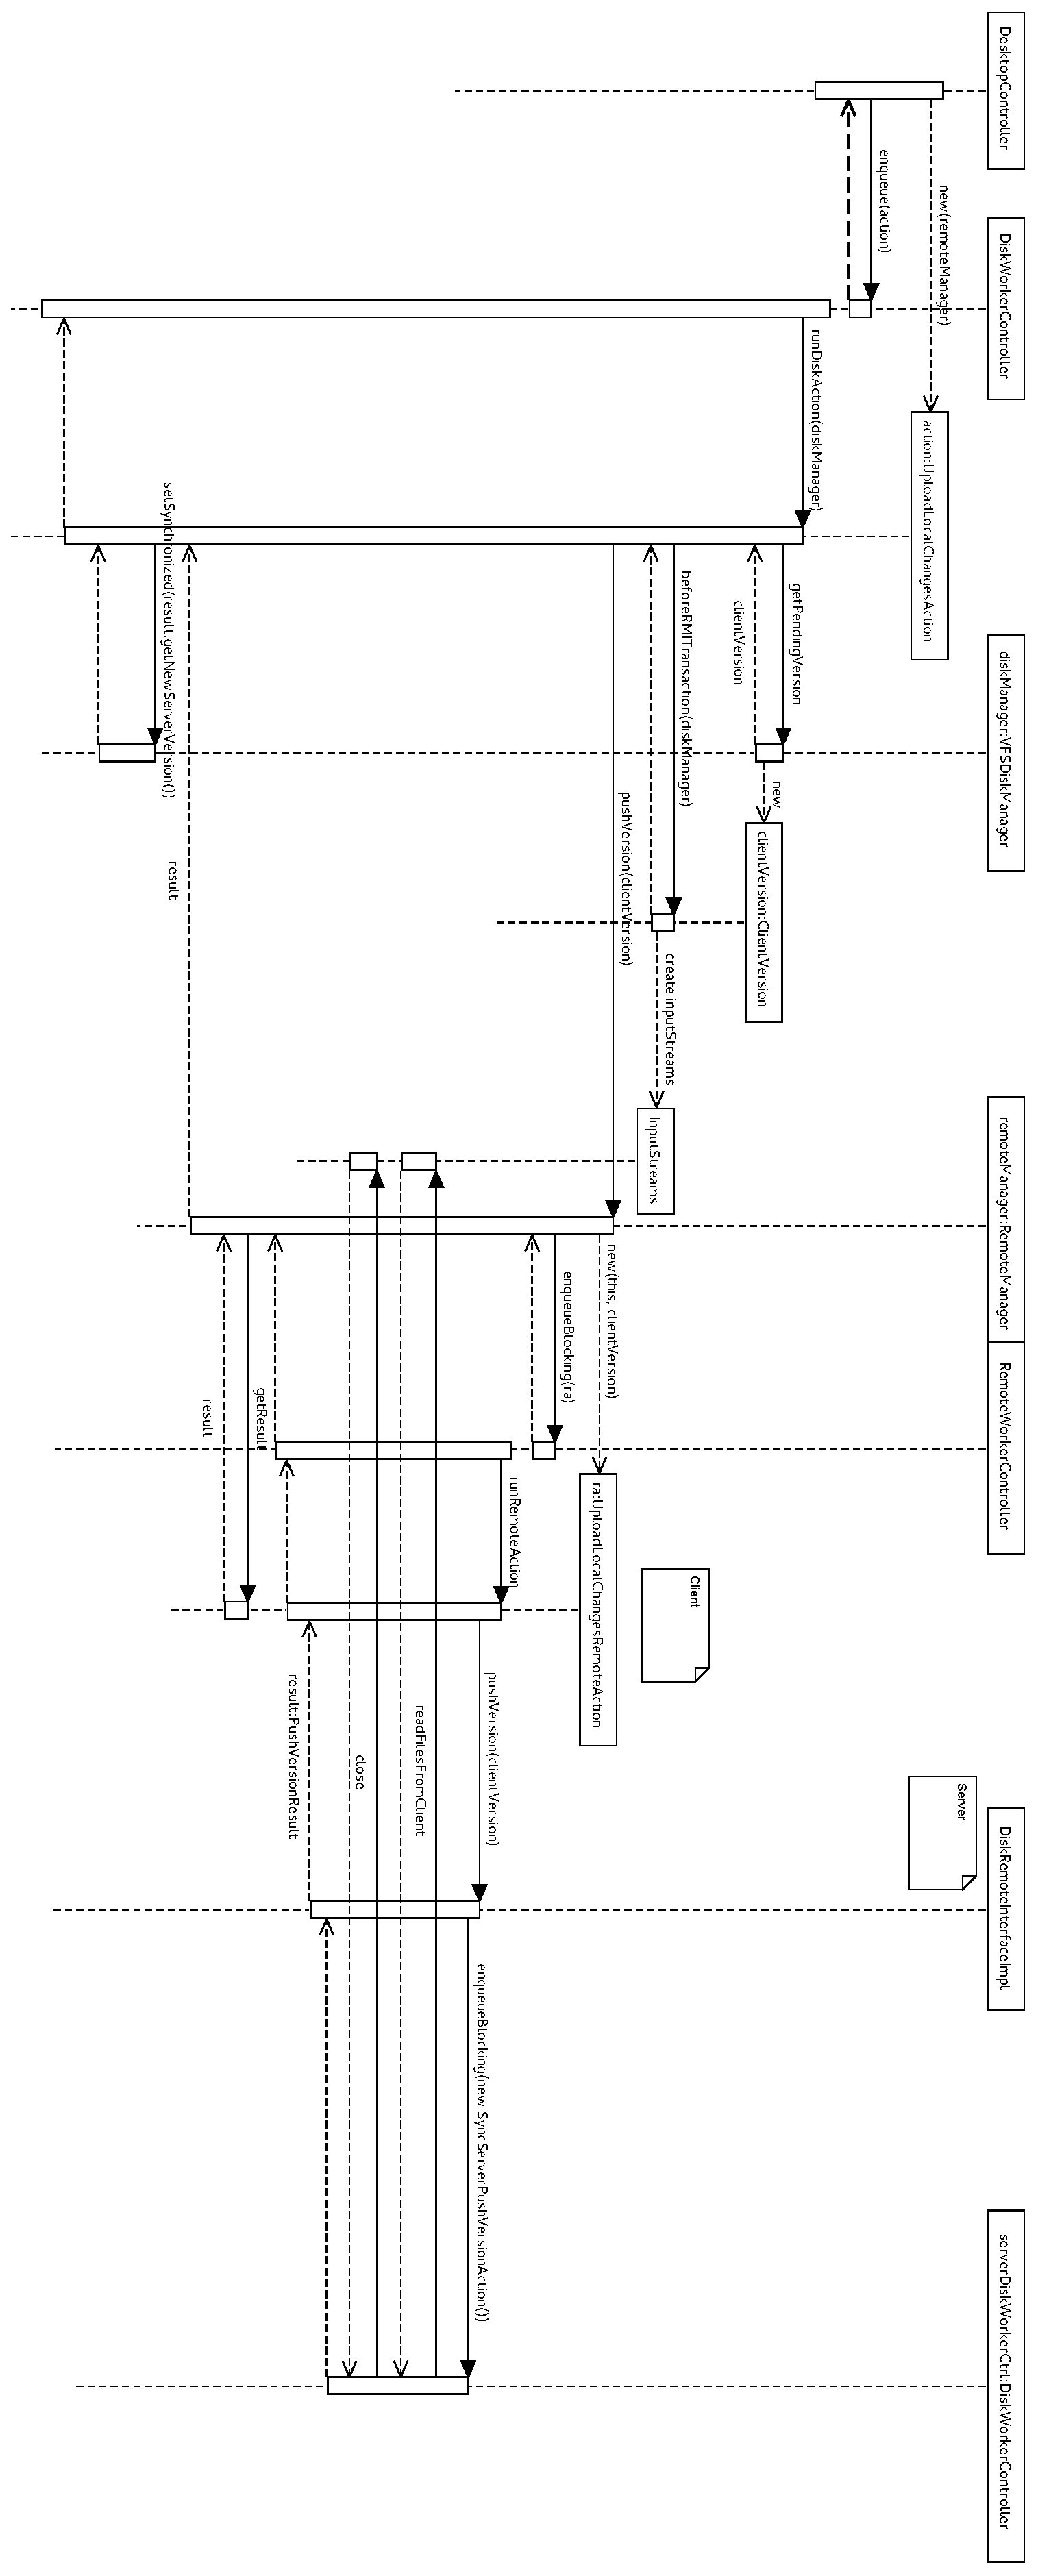
\includegraphics[height=\textheight,width=\textwidth,keepaspectratio]{figures/22uploadChanges.eps}
\caption{from click to upload changes to server}
\label{fig:22uploadChanges}
\end{figure}

\begin{figure}[h!]
\centering
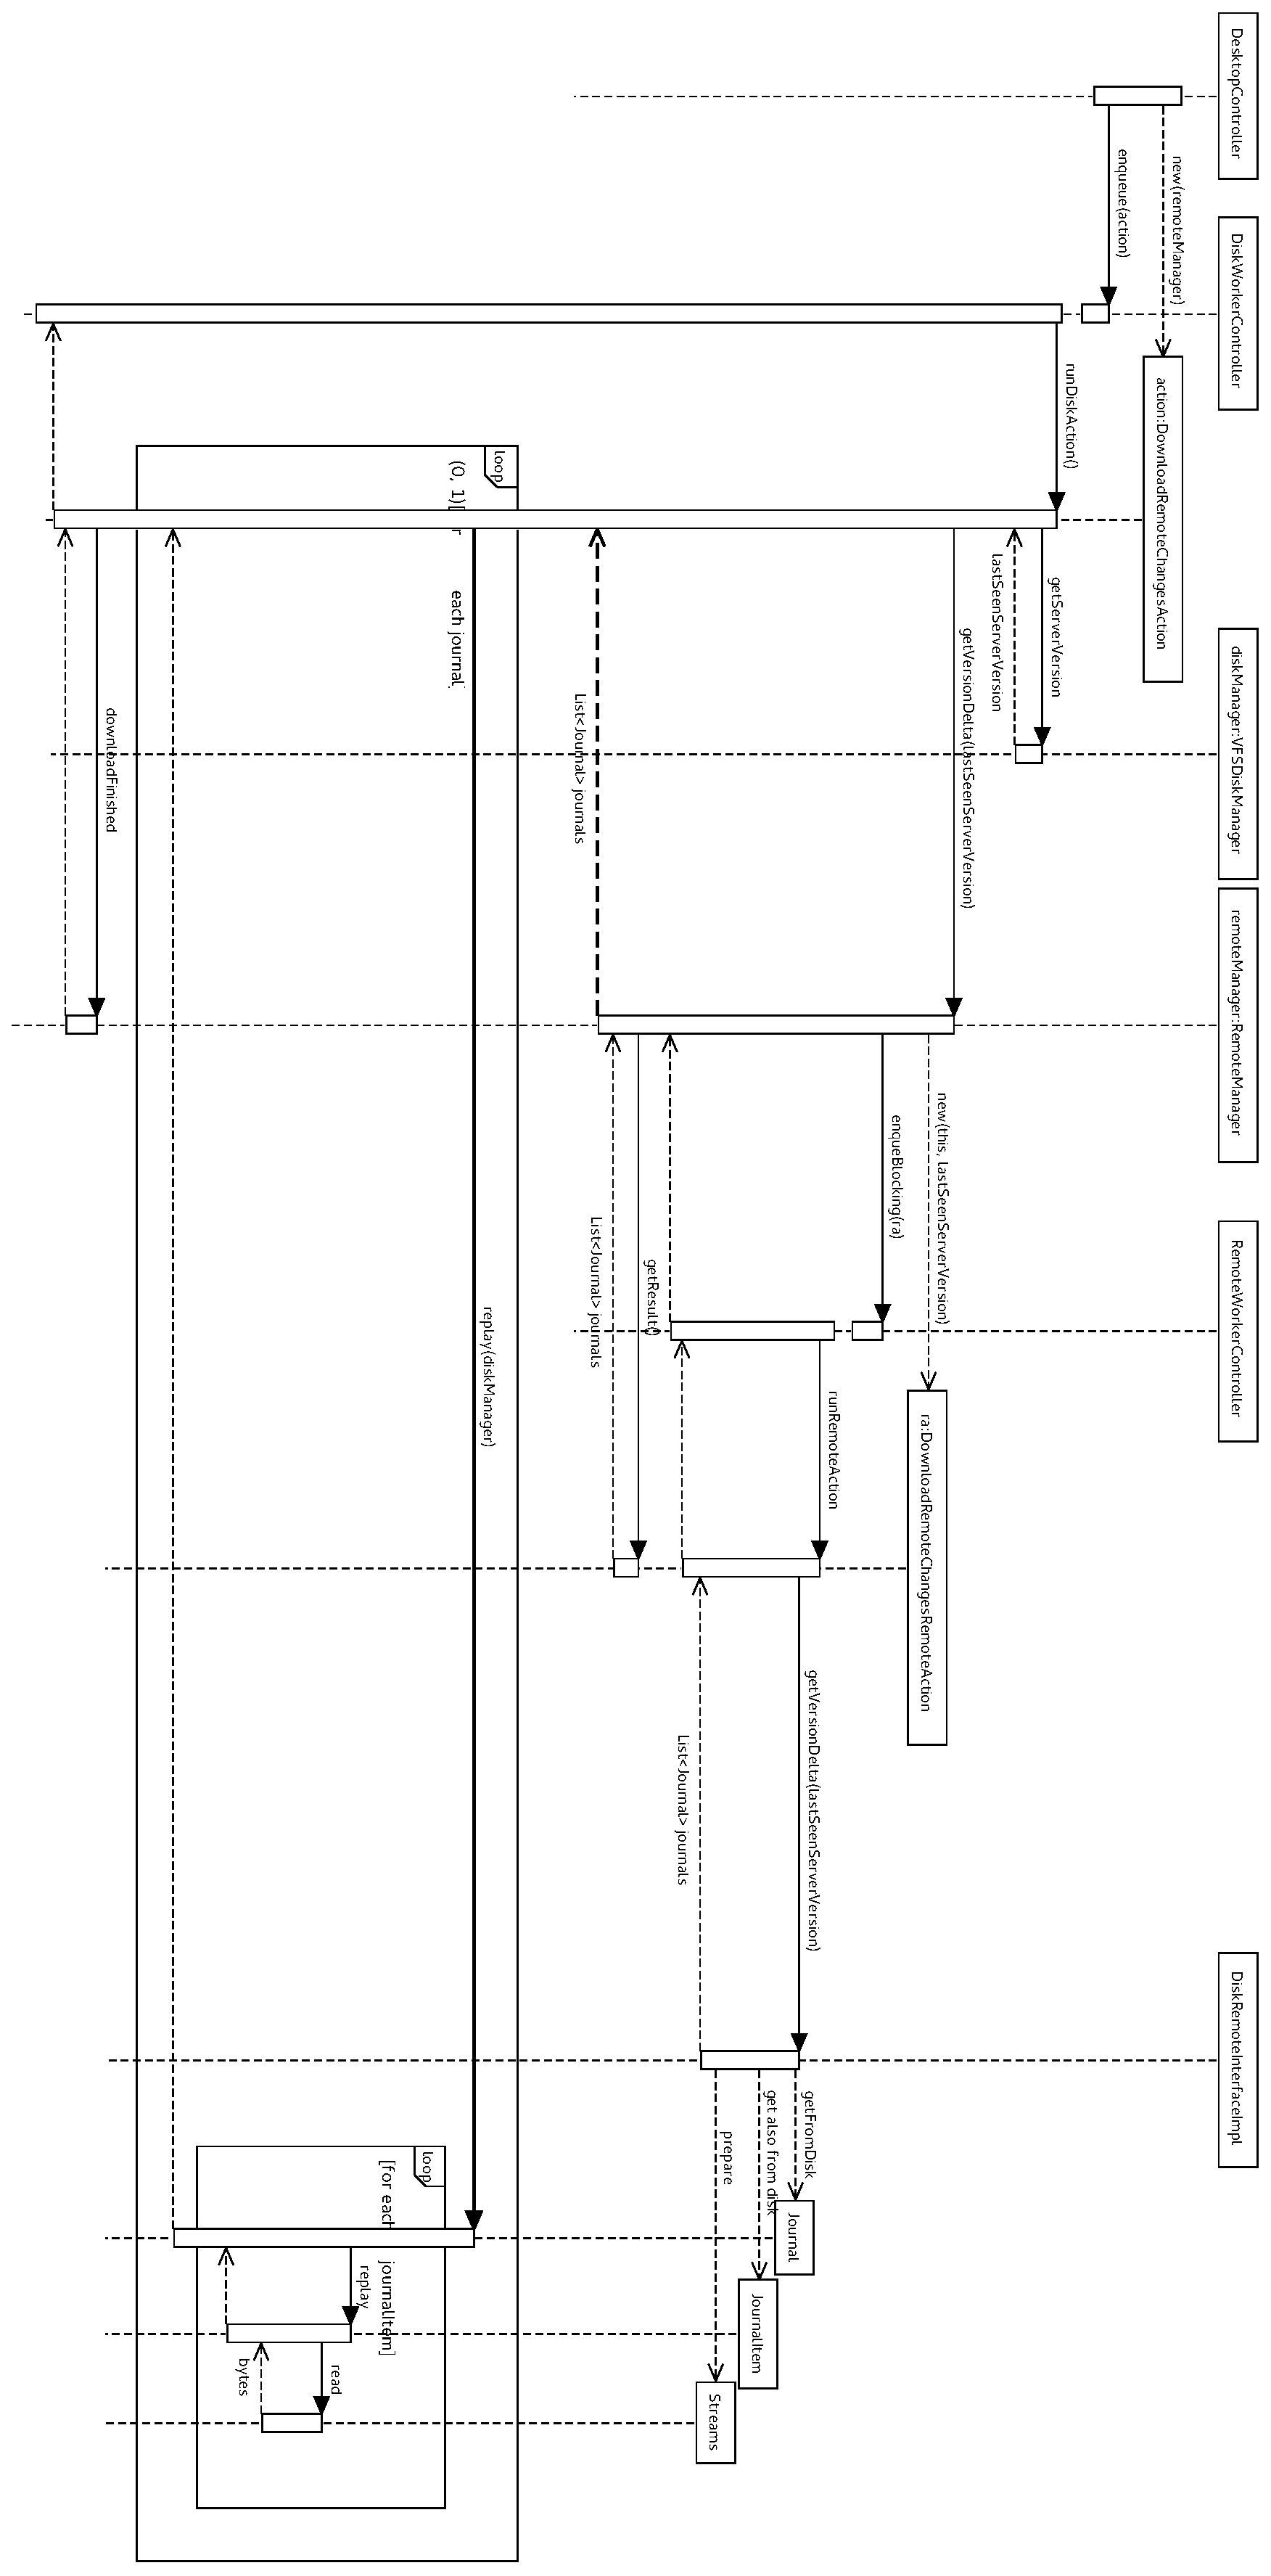
\includegraphics[height=\textheight,width=\textwidth,keepaspectratio]{figures/22downloadChanges.eps}
\caption{from click to download changes from server}
\label{fig:22downloadChanges}
\end{figure}


\subsubsection{longterm polling}
To make other clients aware that changes happened on their disk, a long term
polling mechanism was implemented. Clients start the
\textit{longTermPollVersion} method in the \textit{DiskRemoteInterface}. Upon
files get changed by a client the other clients that are currently connected to
the same disk get notified by returning the \textit{longTermPollVersion} method,
containing the actual server version, to which the clients now have to update.

\subsubsection{Journaling}
Figure \ref{fig:journaling_classes} gives an overview over the classes that
were implemented for journaling. The main thing to notice are the
\textit{JournalItem}s that carry out the operations they represent (e.g.
\textit{RenameEntryItem} renames a given entry to a new one.). For every disk a
logical verion number is kept to make sure that no journals collide. Every time
a client synchronizes the version number that it has last seen gets sent to the
server so that the server can decide which journals have to be propatated to the
client.

 /.hidden/journals/00001/journal.bin
wird durch Journal serialisiert
denn gits /.hidden/Journals/00001/file-09320982309-34234
also /.hidden/journals/[journalnr]/file-[uuid]
de gits shallow copies vo de erzüge files






\begin{figure}[h!]
\centering
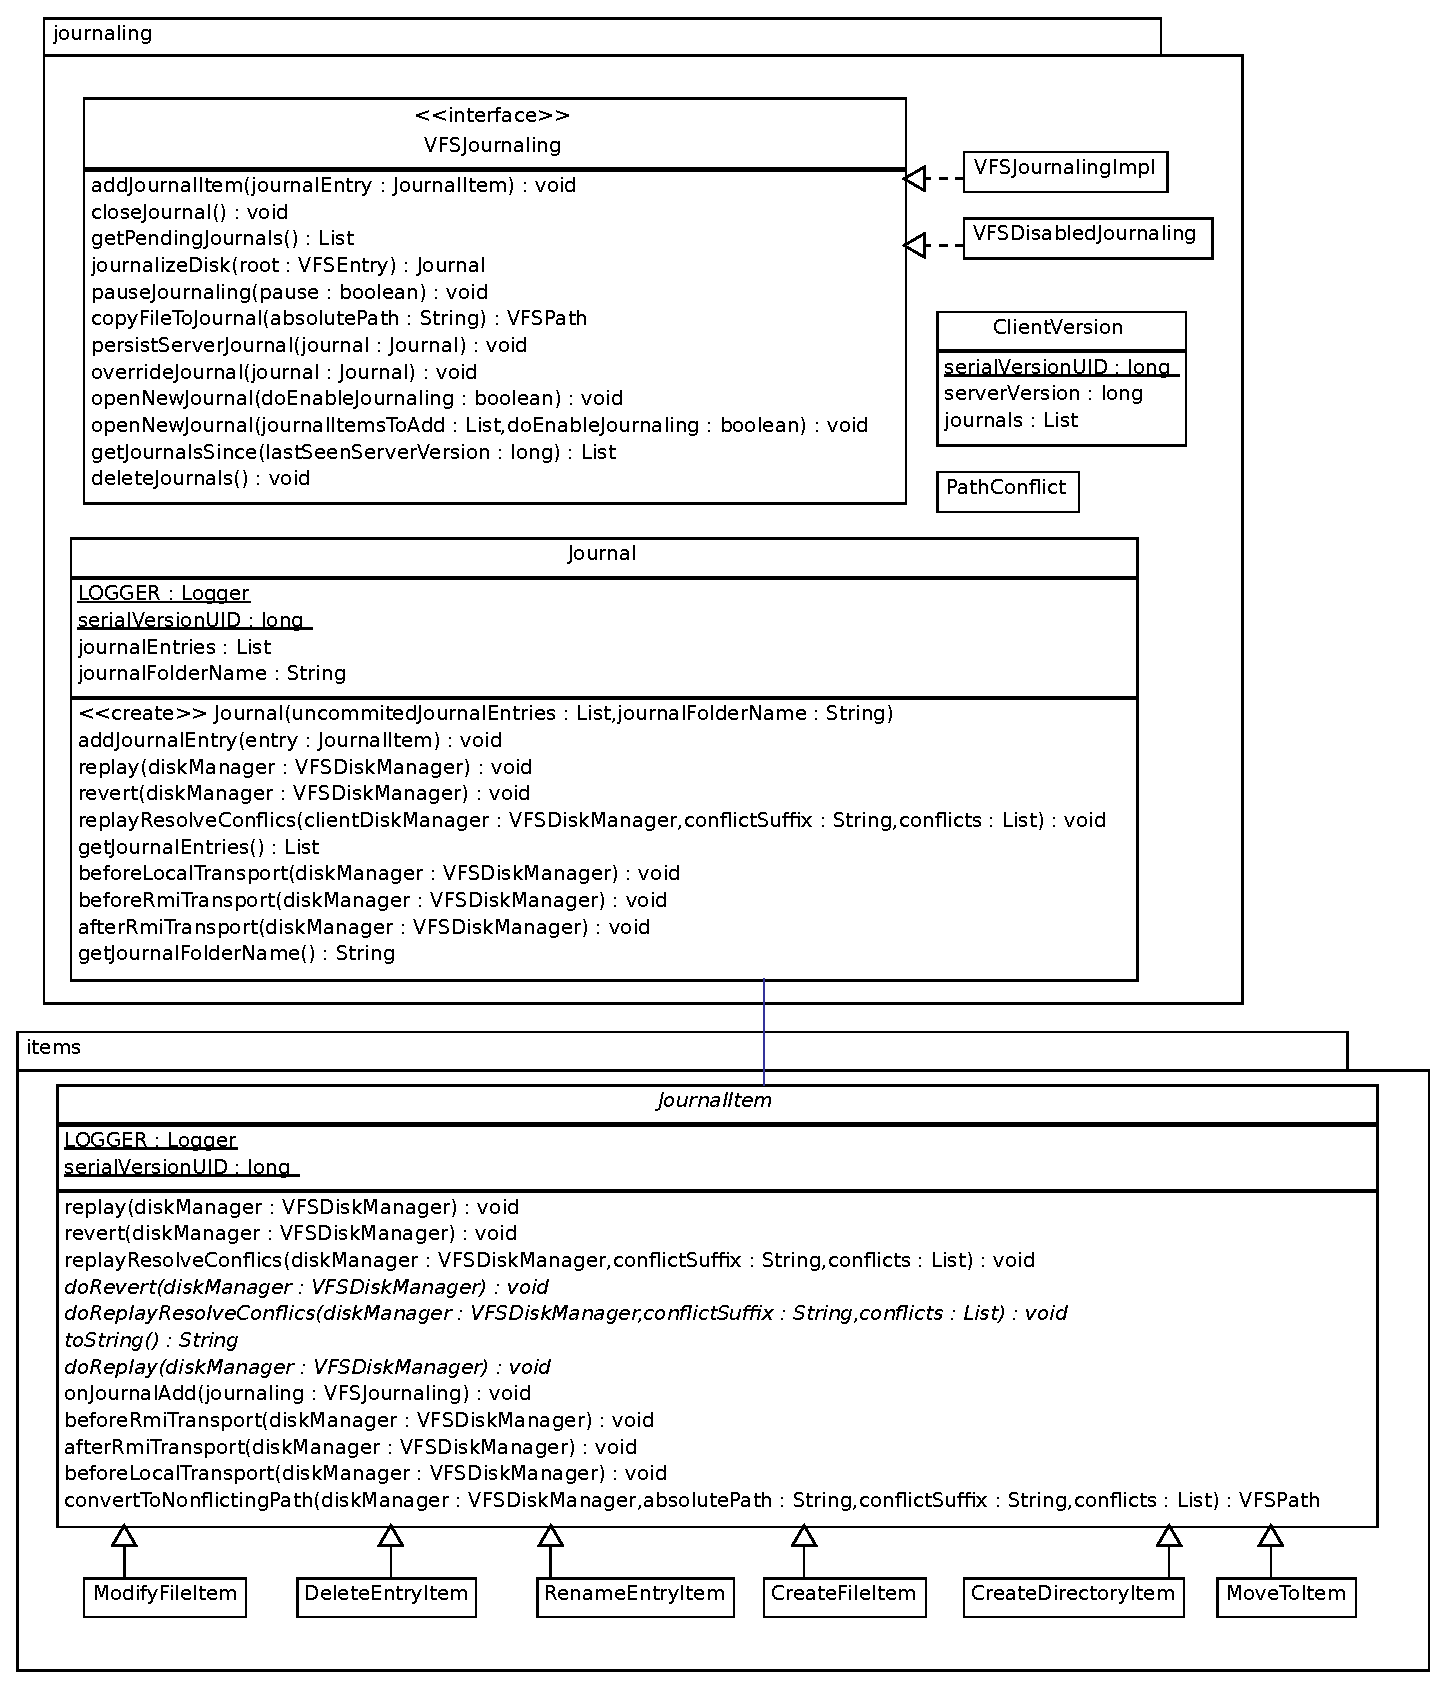
\includegraphics[width=1\textwidth]{figures/22Journaling.eps}
\caption{Journaling classes}
\label{fig:journaling_classes}
\end{figure}

\paragraph{Conflict resolution}
Based on the logical version numbers that are given to each journal the client
is able to do a basic conflict resolution when it detects conflicting changes.
Files that got new content on the server while they were changed locally will be
renamed.

 Matthias:  und conflict resolution isch:
1. revert local changes
2. replay server journal (denn bisch in sync mit em server)
3. redo local changes
4. push local changes to server